\documentclass[problem]{mcs}

\begin{pcomments}
  \pcomment{CP_search_tree}
  \pcomment{DRAFT ARM 2/27/17}
\end{pcomments}

\newcommand{\BST}{\text{BST}}
\newcommand{\sz}[1]{\text{size}(#1)}
\newcommand{\hgt}[1]{\text{height}(#1)}
\newcommand{\srch}[2]{\text{search}(#1,#2)}

\pkeywords{
  recursive
  structural_induction
  search_tree
  tree}

\begin{problem}
Binary search trees are a widely used data type that supports
efficient searching of a large set of ordered items.  For
definiteness, we choose our items to be real numbers.  The set
\BST\ of binary search trees is defined recursively.

\begin{definition*}
\inductioncase{Base case}: A number $r \in reals$ is a \BST, with
\begin{align*}
\min(r) & \eqdef r,\\
\max(r) & \eqdef r.
\end{align*}

\inductioncase{Constructor case}: If $T,U$ are \BST's, $r \in reals$, and
\[
\max{T} \leq r \leq \min{U},
\]
then $\ang{T,r,U}$ is a \BST.  The number $r$ is called the
\emph{root-label} of the constructed tree, and $T$ and $U$ are
respectively the \emph{left} and \emph{right} subtrees of the
constructed tree.
\end{definition*}

The tree $\ang{T,r,U}$ would usually be illustrated graphically as
in Figure~\ref{fig:recBST}.
\begin{figure}
  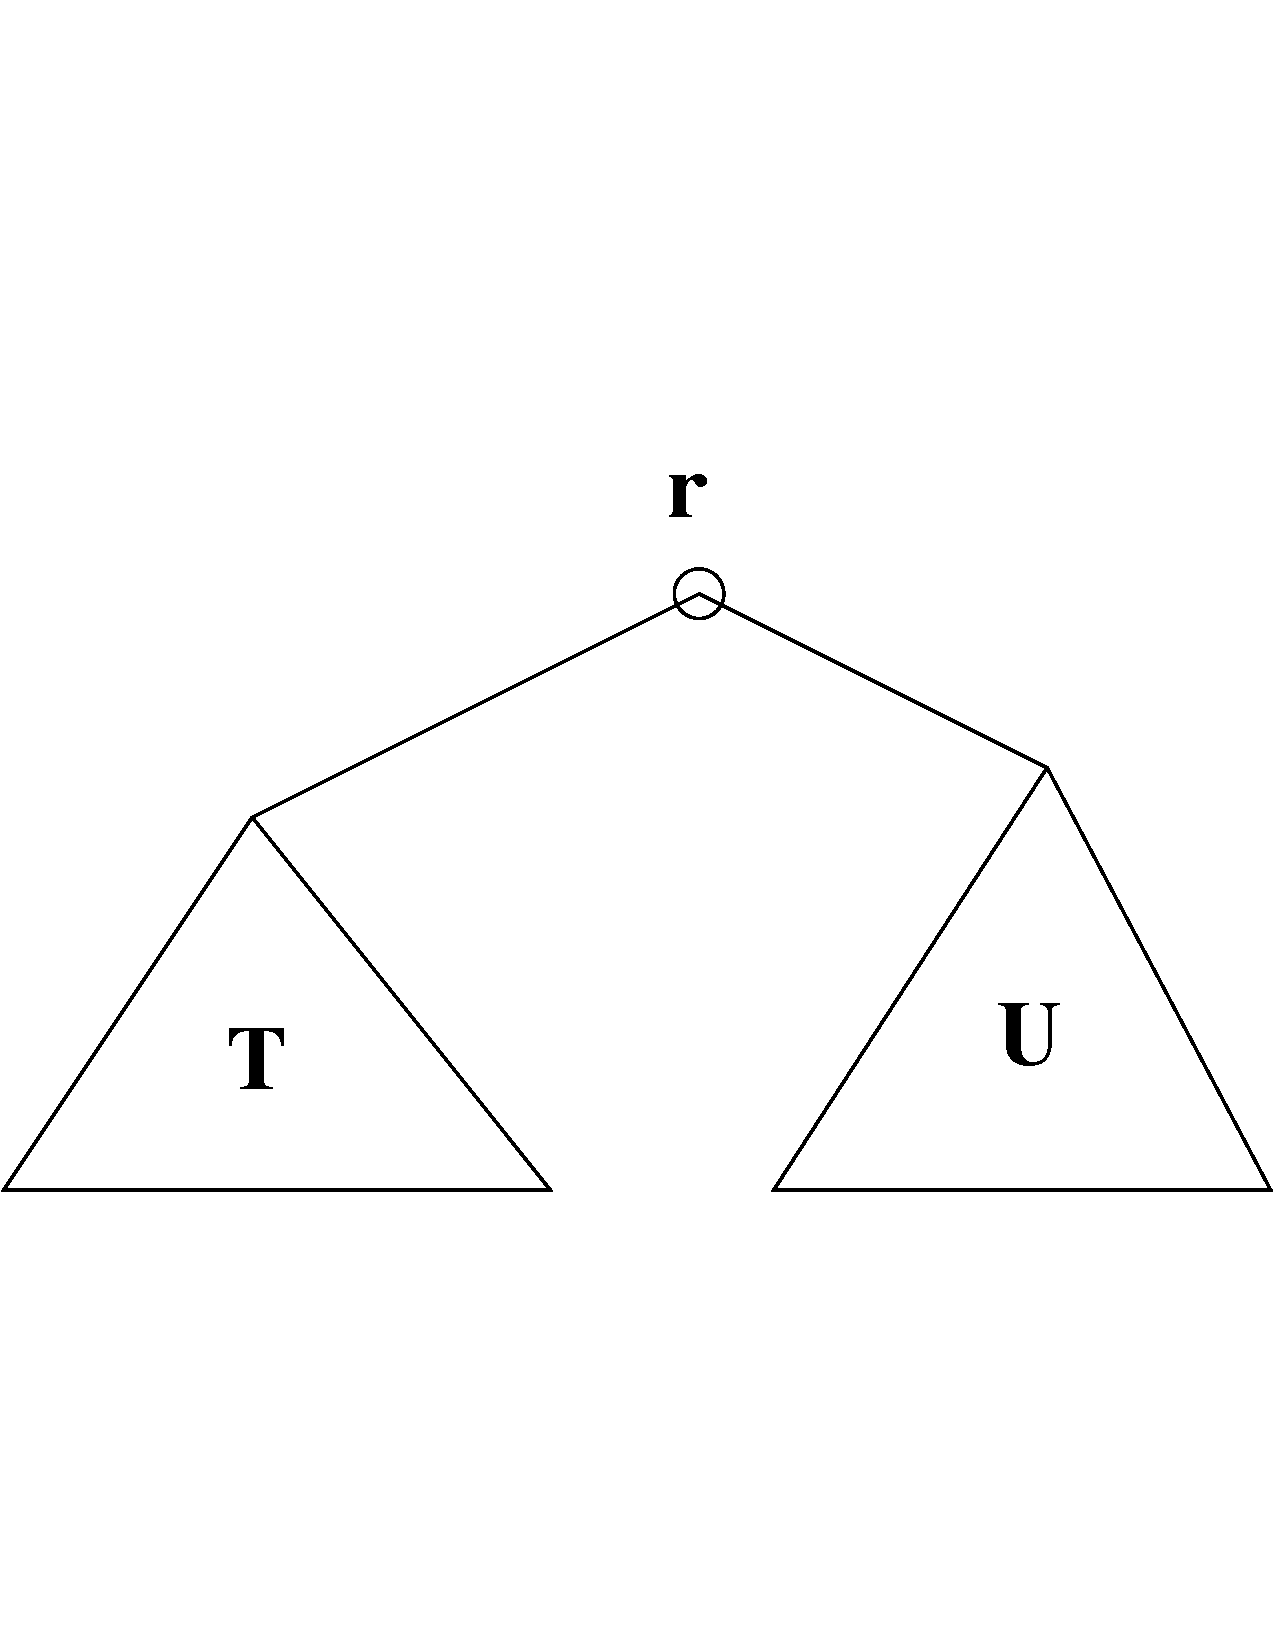
\includegraphics[height=2.0in]{recBST}
  \caption{\BST\ Constructor.}
  \label{fig:recBST}
\end{figure}
A sample \BST\ is shown in Figure~\ref{fig:search-1-7}
\begin{figure}
  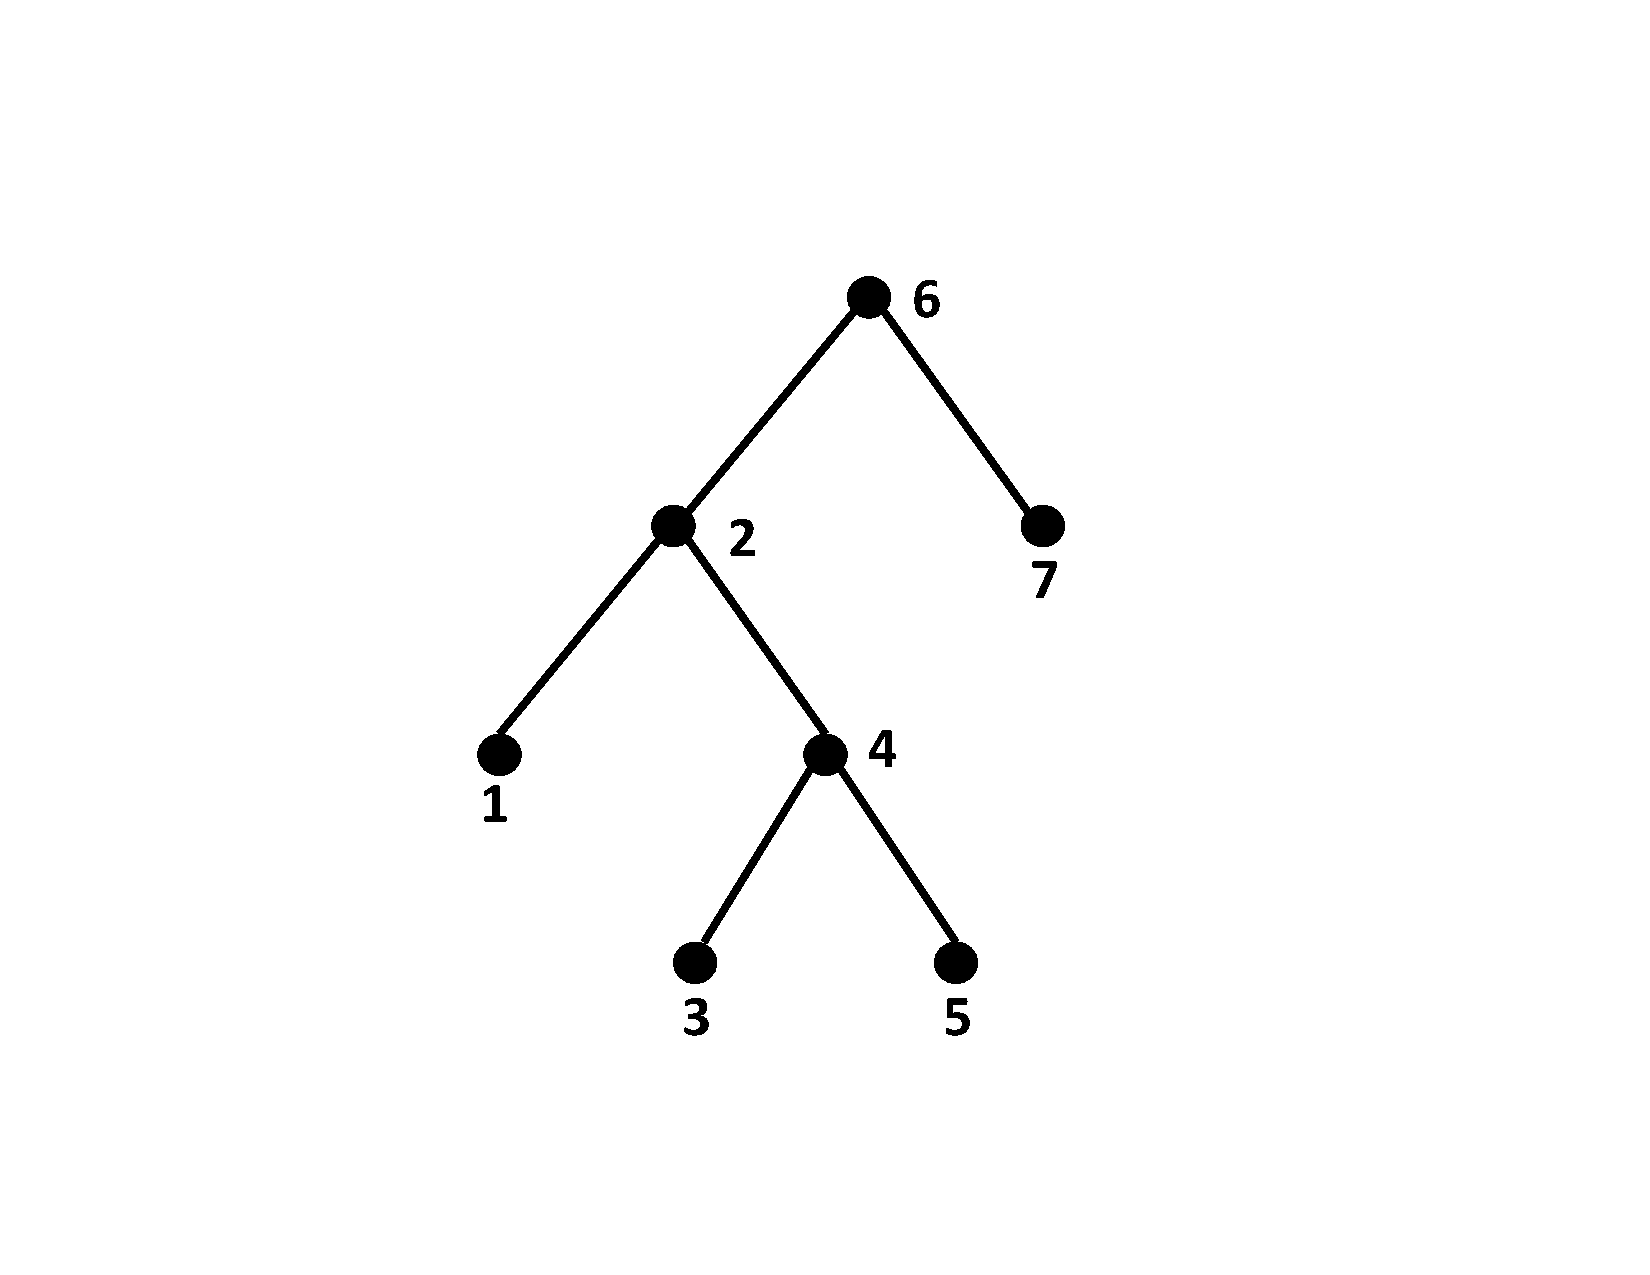
\includegraphics[height=2.0in]{search-tree1-7}
  \caption{A \BST\ for the Integer Interval $\Zintv{1}{7}$.}
  \label{fig:search-1-7}
\end{figure}

\bparts

\ppart Give a recursive definition of the function $\sz:\BST \to \nngint$ where
\begin{align*}
\sz{T} \eqdef \text{\#nodes in}\ T,\\
\hgt{T} \eqdef \text{\#nodes in longest top to bottom path in}\ T.
\end{align*}

\ppart Prove that if $\hgt{T} = h$, then $\sz{T} \leq 2^h - 1$.

\ppart Prove that if $\sz{T} = n$, then 
\[
\ceil{\log_2(n+1)} \leq \hgt{T} \leq n.
\]
Describe a \BST\ of size $n$ with height $n$.  This shows that the
upper bound $n$ on height cannot be improved.  Explain why the lower
bound $\ceil{\log_2(n+1)}$\inhandout{\footnote{$\ceil{r}$ is $r$
    rounded up to the nearest integer.}} cannot be improved either.

\ppart Name subtrees by LRLLR-type path to them from root.  Give a
recursive def of the subtree defined by a path.

\ppart Give a recursive definition of a function
\[
\text{search}:(\reals \cross\BST) \to \set{L,R}^* \union{\text{fail}}
\]
such that $\srch{r}{T}$ is a path to a subtree in $T$ whose root-label
is $r$.  If there is no such subtree, then $\srch{r}{T} \eqdef
\text{fail}$.

\end{problem}

\endinput
